
\documentclass[10pt,twocolumn,letter]{article}
\usepackage{styles/usenix-style}
\usepackage[american]{babel}
\usepackage{amssymb}
\usepackage{amsfonts}

%\usepackage{styles/ieee-style}

\author{Adrian E. Lehmann}
%\affiliation{System Architecture Group\\ University of Karlsruhe, Germany}
%\email{adrian.lehmann@student.kit.edu}

%%%%%%%%%%%%%%%%%% Document %%%%%%%%%%%%%%%%%%%%%%%%%%%%%%%%%%%%%%%%%%%
%\usepackage[draft]{styles/ka-style}
\usepackage{cite,xspace,ifthen,graphicx,listings}
%\usepackage[draft]{styles/ka-style}
\usepackage[super]{nth}
\usepackage{theorem}
\usepackage[dvipsnames,table]{xcolor}
\usepackage{tikz}
\usetikzlibrary{decorations.pathreplacing}
\usetikzlibrary{shapes.geometric}
\usetikzlibrary{matrix,shapes,arrows,positioning,chains}
\usepackage{varwidth}
\usepackage{float}
\usepackage{microtype}
\usepackage{tabularx}

\usepackage[all]{nowidow}

\usepackage[
   pdfauthor={Adrian E. Lehmann},
   pdftitle={NTFS},
   pdfsubject={Windows Internal Introductory Seminar},
   pdfkeywords={Filesystem, Windows}
]{hyperref}

\begin{document}

\title{New Technology File System (NTFS)}
\newcommand{\todo}[1]{{\texttt{[#1]}}}
\newcommand{\code}[1]{{\tt \small{#1}}}
\newcommand{\bplus}{B\textsuperscript{+}}
\newcommand{\logn}{$\mathcal{O}(\log{}n)$}
\maketitle
%\draftfooter

% !TeX root = ntfs.tex
\begin{abstract}
The New Technology File System (NTFS) provides a reliable way to store and organize files. In order to accomplish this it divides up the disk into small units called ``Clusters'' which can be individually addressed.\\
To organize files and  directories NTFS has a big table index structure called the Master File Table (MFT). This table stores or references all the (meta-)data of a given file. Directories are stored just like files only that the data they contain is references to files and directories.\\
For the case of a system crash NTFS has further devised a system called ``Journaling'' that logs all the changes  to the drive and ensures these changes are stored fully completed on the disk in case of such a crash.
\end{abstract}
% !TeX root = ntfs.tex
\section{Introduction}
Computers have always been used as a tool for storing and accessing information. One could argue they act as a form of digital library. A centralized place which contains a plenitude of data.
Though just having data does not do much good. It needs to quickly accessible when needed. As of such there  needs to be a form of organization. What in the context of a library might be an indexing system, is a file system to a computer.\\
A file system ensures quick and organized access to data without needing to be familiar with the underlying storage medium (e.g., solid state disk, hard drive, or tape drive).
Furthermore a file system should be resilient to system crashes, which essentially means preventing corruption of the file system, as this would inevitably lead to data loss.\\
Being an integral part of computing a file system is a core component of all modern operating systems, including Microsoft Windows. Since 1993\cite{Custer:1994:IWN} Microsoft has shipped all desktop and server Windows operating systems with a file system called \textit{New Technology File System} (\textit{NTFS}). In the following paper we will take a closer look at how NTFS achieves the aforementioned requirements for a file system: First it will be described how NTFS lays out the available storage in section \ref{sec:Cluster}, after which the data structure for organizing stored data will be looked at in section \ref{sec:MFT}. Lastly the resilience aspect of NTFS will be highlighted in section \ref{sec:Recovery}.
% !TeX root = ntfs.tex
\section{Addressing Storage: Clustering}
\label{sec:Cluster}
Before we can begin to organize files, we first need to be able to manage the available space. In order to divide up the storage medium NTFS has implemented a system called \textit{clustering} \cite{RUSSINOVICH_ET_AL:2012:WI}.

The basic idea of clustering is to divide up the storage medium into contiguous parts, called \textit{clusters}. These clusters are made up of $2^n, n \in \mathbb{N}$\cite{microsoftinc:2018:DCS} sectors (usually sized $4096$ Bytes \cite{bibid}) on a storage device and hence abstract from the physical layout. When formatting a volume the size of clusters can be set, but it cannot be changed afterwards without formatting again\cite{RUSSINOVICH_ET_AL:2012:WI}.\\
Setting the cluster size seems at first glance like an arbitrary choice, but it is not. It is a trade-off between internal fragmentation and speed:
When increasing the cluster size there is less management overhead for the clusters as there is fewer of them. The reduced overhead will improve speed.\cite{RUSSINOVICH_ET_AL:2012:WI} Further, as the clusters being mapped to contiguous blocks the speed of access is also improved with larger cluster sizes. Especially for media with mechanical parts accessing contiguous memory this is a lot faster due to less mechanical movement of the read/write head being required. As for solid state memory contiguous access still provides speed benefits, because SSDs do not load one block at a time, but rather a collection of consecutive blocks.\cite{BELLOSA:2017:OS}
At the same time though, when larger cluster sizes are set there is potential for clusters only partially containing actual data and hence potential for higher internal fragmentation. Furthermore, as NTFS addresses clusters using 32-bit addresses, there is a theoretical limit to how large a drive can be with a given cluster size.\cite{hughes:2010:UT2}

%In figures \ref{fig:internal_frag_16} and \ref{fig:internal_frag_4} this is illustrated. In this example we are storing 2 KiB of data in a cluster. With the cluster size set to 4 KiB (figure \ref{fig:internal_frag_4}) we can see that we have less space that cannot be used due to our memory allocation compared to the cluster size set to 16 KiB (figure \ref{fig:internal_frag_16}). Specifically when using the 4 KiB clusters we lose $50\%$ of the allocated storage to internal fragmentation, whereas for the 16 KiB clusters we lose $87.5\%$.
%\begin{figure}[H]
%	\centering
%	\fbox{
%		\resizebox {0.95\columnwidth} {!} {
%			\begin{tikzpicture}[scale=1]
%				\filldraw [fill=SpringGreen, draw=black] (0,0) rectangle +(1,2);
%				\filldraw [fill=white, draw=black] (1,0) rectangle +(7,2);
%				\draw [decorate,decoration={brace,amplitude=6pt,mirror,raise=1pt},xshift=0pt,yshift=-4pt,font=\footnotesize,align=center]
%				(0.1,0) -- (0.9,0) node [black,midway,yshift=-0.6cm]
%				{$2$ KiB\\used};
%				\draw [decorate,decoration={brace,amplitude=6pt,mirror,raise=1pt},xshift=0pt,yshift=-4pt,font=\footnotesize,align=center]
%				(1.1,0) -- (7.9,0) node [black,midway,yshift=-0.6cm] 
%				{$6$ KiB unused};
%			\end{tikzpicture}
%		}
%	}
%	\caption{Illustration of internal fragmentation: Cluster size 16 KiB\label{fig:internal_frag_16}}
%\end{figure}
%\begin{figure}[H]
%	\centering
%	\fbox{
%		\resizebox {0.95\columnwidth} {!} {
%			\begin{tikzpicture}[scale=1]
%				\filldraw [fill=SpringGreen, draw=black] (0,0) rectangle +(4,2);
%				\filldraw [fill=white, draw=black] (4,0) rectangle +(4,2);
%				\draw [decorate,decoration={brace,amplitude=6pt,mirror,raise=1pt},xshift=0pt,yshift=-4pt,font=\footnotesize,align=center]
%				(0.1,0) -- (3.9,0) node [black,midway,yshift=-0.6cm]
%				{$4$ KiB used};
%				\draw [decorate,decoration={brace,amplitude=6pt,mirror,raise=1pt},xshift=0pt,yshift=-4pt,font=\footnotesize,align=center]
%				(4.1,0) -- (7.9,0) node [black,midway,yshift=-0.6cm] 
%				{$4$ KiB unused};
%			\end{tikzpicture}
%		}
%	}
%	\caption{Illustration of internal fragmentation: Cluster size 4 KiB\label{fig:internal_frag_4}}
%\end{figure}
By default Microsoft has set the cluster size for usual desktop storage capacities (2GB - 16TB) to $4$ KiB \cite{microsoftinc:2018:DCS}. For larger storage needs the default cluster size is greater than $4$ KiB. In these instances one would usually not worry about internal fragmentation on a kilobyte-level, but due to the addressing limitation, drives larger than 16TB must use clusters larger than $4$ KiB.

\subsection{Virtual and Logical Clusters}
\label{sec:Cluster:CN}
Now that we have established that clusters are just some unit of memory lets look at how to address them. \\
For this we need to distinguish between \textit{logical} and \textit{virtual} clusters:
\begin{itemize}
	\item Logical clusters are the physical collections of \textit{sectors} on a disk 
	\item Virtual clusters are the clusters that are used within a given file
\end{itemize}
So the name space of virtual clusters is file local, whereas the name space of logical clusters is global. This does not mean though that virtual and logical clusters are independent. Virtual cluster. Virtual clusters are another layer of indirection for addressing disk space.
One of the reasons for this is that with many programs reading and writing data at the same time collisions would be bound to happen. As of such each file can be treated as its own ``virtual'' file system. This allows for programs to be able to manage the file they are writing to and not have to worry about other files on the disk and interfering with them. This system is very similar to the idea of virtual and physical memory, only clustering is in terms of non-volatile storage.
%TODO: Go deeper!
This allows for sparse files, i.e. files that are mostly empty, to not occupy a lot of disk space, as their empty clusters are not mapped to physical clusters. efficiency.\cite{RUSSINOVICH_ET_AL:2012:WI}\\
Virtual clusters are referenced by Virtual Cluster Numbers (VCNs). The first VCN of a file always has an index of $0$ and every other VCN indicates the offset from the beginning of the file. 

Logical Cluster Numbers (LCNs) on the other hand are indices for logical clusters and represent the offset from a given (arbitrary, but constant) point on the medium, which has been assigned LCN $0$.\cite{RUSSINOVICH_ET_AL:2012:WI}
In summary logical and virtual cluster numbers are concepts that coexist to address clusters easily within the different domains of media and files.
% !TeX root = ntfs.tex
\section{Master File Table (MFT)}
\label{sec:MFT}
After analyzing how NTFS actually addresses storage, we will now look at how NTFS organizes the now available and addressable storage space. Like most modern file systems NTFS allow for organizing data using files and hierarchical directories. But with this structure there come some challenges: Where to store (meta-)data, the amount of files, that the depth of directories should not be limited, and a lot more. In the following section we will take a look at how NTFS aims to solve these problems.\\

% MFT Table -> What's in there -> Files -> Extents -> Directories -> Bitmap -> Extends -> Big Picture & Redundancy

\begin{figure}[h]
	\centering
	\fbox{
		\begin{tabularx}{0.95\columnwidth}{|cX|}
			\hline
			0 & \texttt{file or directory} \\
			\hline
			1 & \texttt{file or directory} \\
			\hline
			2 & \texttt{file or directory} \\
			\hline
			... & \\
			\hline
		\end{tabularx}
	}
	\caption{Conceptual design of MFT\label{fig:mft_concept}}
\end{figure}
In order to have a directory of files and directories, NTFS has a table-like structure, called the \textit{Master File Table} (\textit{MFT}). In this table, most rows will represent a single file or directory entry (technically the first few rows are different, but that shall not be in the scope of this report). This has been schematically illustrated in figure \ref{fig:mft_concept}. Before we get to how files and directories are stored, we will just take a look at how the MFT grows. The MFT is a file itself (and thus referenced within itself), located at \texttt{C:\textbackslash\$MFT}\footnote{Drive letter might differ}.\cite{RUSSINOVICH_ET_AL:2012:WI} As there is no predetermined maximum of files and directories that can be stored, the MFT needs to be able to grow dynamically. As the lookup times in the MFT should be rather low NTFS makes sure that whilst the MFT can grow that it is kept as contiguously stored on disk as possible. In order to do this NTFS will at first allocate $12.5\%$ of the available disk space and the release unused space, only once the disk has filled far enough for the space to be required. If the reserved amount of space should ever be exceed, more space will be allocated at a non-contiguous part of the disk. Unfortunately, due to MFT elements being referenced from potentially multiple places within the MFT, defragmentation cannot move MFT elements.\cite{microsoftinc:2018:HNR}. With all of this said, on a system with ``regular'' desktop usage the MFT is relatively small. On a volume with 500GB in use, the MFT size was approx. 1GB ($0.2$\% of total disk space).\\  Now that we know how the MFT grows, let's look at the data that actually occupies it. Generally a MFT Entry is represents one of two things: A file\footnote{N.B.: Windows, and hence NTFS do not employ the ``\textit{everything is a file}''-paradigm} or a directory. In the following we take a closer look at the structure of the aforementioned entry types.\\
\subsection{Storing files}
When it comes to files there is a lot of data that we would like to store: The actual data of the file, a filename, the creation date, the folder it is in and a lot more. Depending on the file though we might not always want to store the same metadata though. In order to account for this the MFT is not a table in a strict sense, as it does not have fixed columns in which data can be stored. Rather it works based on a concept called streams. Streams are, as the name suggest, just sequences of bytes. In order to enable full flexibility a MFT-Record can store an arbitrary amount of streams, that can contain various pieces of (meta-)data. In the following we will be taking a look at a few very common streams, the data they contain and how streams themselves are stored. Something interesting to note is that not only metadata, but also the actual data of a file is strictly speaking a stream. In figure \ref{fig:mft_entry} the layout of an example file with common data streams is shown. In the following we will look at the data streams that have been shown in figure \ref{fig:mft_entry}.
\begin{figure}[H]
	\centering
	\fbox{
		\begin{varwidth}{0.95\columnwidth}
			\begin{tabularx}{0.95\columnwidth}{|c|c|c}
				\hline
				Standard information & File name & $\hookrightarrow$ \\
				\hline
			\end{tabularx}
			\newline	
			\vspace{1pt}
			\newline
			\begin{tabularx}{0.95\columnwidth}{c|c|c|c}
				\hline
				$\hookrightarrow$ & Security descriptor  & Data & ...\\
				\hline
			\end{tabularx}
		\end{varwidth}
	}
	\caption{Example MFT file entry\label{fig:mft_entry}}
\end{figure}
The first attribute is always present in a file entry: \texttt{\$STANDARD\_INFORMATION}. This stream contains information such as \textit{read-only}, \textit{last-modified} and \textit{creation-time}. This data is important for any file an will hence always be present in an MFT entry.\cite{RUSSINOVICH_ET_AL:2012:WI}\\
The \texttt{\$FILE\_NAME} is a unicode\footnote{Excuding unicode characters reserved for other purposes, e.g., \texttt{\textbackslash}} name, which can have store as many as 255 characters.\cite{microsoftinc:2018:MFP} This is a limitation that serves to ensure that a  file name is  short enough to fit within an entry.
As security is out of scope for this paper we will not go to deep into the \texttt{security descriptor}. In short we can say  the attribute is used for access control.
Lastly the most interesting part of the a file. The \texttt{data}. In this stream all of the corresponding data to a file can be found.\\
%TODO: Rework next paragraph 
All of these attributes are part of our MFT entry. In a perfect world all of this data would just be kept within the MFT entry, but due to the sheer size of some files, the variability of possible streams stored and the fact that an MFT entry is only a fixed size (usually 1 KB\cite{B:2017:AJI}), at some point (meta-)data will need to be stored outside of the MFT. Up until the maximum record size is reached, all streams can be stored within the MFT record and can  be accessed very quickly.
\subsection{Referencing data}
As soon as the streams of a file exceed the given size limit, the Data stream of the file will be stored outside of the MFT. In order to accomplish this the data outside of the MFT is referenced (think of pointers for now). In the beginning of this report in section \ref{sec:Cluster}, we studied Clustering and how we can use it to address storage on the volume. With this information in mind the first naive idea would be to use as many clusters as we need, wherever they are free and store cluster numbers as ``pointers'' to each of them in the MFT entry. But unfortunately if we think of a very large file, the sheer number of pointers and the accompanying storage requirement would by far exceed feasibility. Hence NTFS is not referencing individual clusters, but rather multiple chunks of contiguous clusters, called extents. Extents are represented as a 3-tuple containing, the starting VCN, starting LCN and length. From the cluster identified by the starting VCN and LCN onwards, $l$ clusters are in the given extent. This means an extent $(s_v, s_l, l)$ is representing the following clusters:
\begin{center}
	$\{(c_v, c_l) \mid c_v, c_l \in \mathbb{N} \wedge c_v \in [s_v, s_v + l] \wedge c_l \in [s_l, s_l + l]\}$
\end{center}
where $c_v$ is the VCN and $c_l$ the LCN.\cite{miller:2013:CNS} An example of how to interpret an extent can be seen in figure \ref{fig:extent_basic}. In this figure the extent identified by the 3-tuple $(20, 60, 2)$, which means it has a length of two clusters and starts a the cluster identified VCN 20 and LCN 60. Hence the clusters $(20, 60)$ and $(21, 61)$ would be in the given extent and are marked green in the figure \ref{fig:extent_basic}.
\begin{figure}[h]
	\centering
	\fbox{
		\begin{varwidth}{0.95\columnwidth}
			Extent description:
			\newline
			\vspace{0.25pt}
			\begin{tabularx}{0.95\columnwidth}{|X|X|X|}
				\hline
				Start VCN & Start LCN & Length\\
				\hline
				20 & 60 & 2\\
				\hline
			\end{tabularx}
			\newline	
			\vspace{1pt}
			\newline
			Resulting cluster usage:
			\newline
			\vspace{0.25pt}
			\begin{tabularx}{0.95\columnwidth}{|X|X|X|X|X|}
				\hline
				\textbf{LCN} & 59 & \cellcolor{SpringGreen}60 & \cellcolor{SpringGreen}61 & 62 \\
				\textbf{VCN} & / & \cellcolor{SpringGreen}20 & \cellcolor{SpringGreen}21 & / \\
				\hline
			\end{tabularx}
		\end{varwidth}
	}
	\caption{Example Extent\label{fig:extent_basic}}
\end{figure}
Going back to the problem of storing data outside of the MFT: NTFS will instead of referencing individuals cluster, as previously mentioned, extents. So if a file has a certain storage requirement NTFS will look for empty clusters and group contiguous ones into extents and will then reference these extents in the corresponding MFT entry. In figure \ref{fig:extent_file} an example for this is displayed. In the given example it is showcased how 2 MiB of data could be referenced using extents on a NTFS volume with 4 KiB clusters.
We can see that the total number of clusters in the extents sum up to 512 clusters which is the exact storage requirement. Furthermore we can observe that there is no gap in VCNs, all VCNs 0 through 511 are mapped. Mapping all VCNs from 0 through $n-1$, where $n$ is the number of clusters needed is always required, as VCNs are local to a file and represent offsets from the beginning (See section \ref{sec:Cluster:CN}). On the other hand, logical clusters are spread across the disk without a clear pattern.\cite{RUSSINOVICH_ET_AL:2012:WI} This implies that there might be a high degree of external fragmentation between the individual extents. That said the lack of locality restrictions allow for an easier allocation process and high degree of storage utilization.
\begin{figure}[h]
	\centering
	\fbox{
		\begin{varwidth}{0.95\columnwidth}
			Referenced extents:
			\newline
			\vspace{0pt}
			\newline
			\begin{tabularx}{0.95\columnwidth}{|X|X|X|}
				\hline
				Start VCN & Start LCN & Length\\
				\hline
				0 & 7291 & 256\\
				256 & 14 & 64\\
				320 & 100 & 189\\
				509 & 5 & 3\\
				\hline
			\end{tabularx}
		\end{varwidth}
	}
	\caption{Referenced extents example for a 2 MiB of data with a cluster size of 4 KiB\label{fig:extent_file}}
\end{figure}
\subsection{Directories}
With the ability to store file the challenge of managing a directory structure arises. NTFS stores directories basically just like files, except for the fact that instead of storing data they store the identifiers of files, which can be looked up in the MFT. If all the references fit within an MFT entry then, as with file data, they will be stored in the entry linearly. Next to the identifiers, for the sake of reducing the number of lookups, file size (in number of clusters) and file names are also stored as file indices within the directory, to simplify listing and size computing. An example can be seen in figure \ref{fig:extent_file_indicies}.
\begin{figure}[H]
	\centering
	\fbox{
		\begin{varwidth}{0.95\columnwidth}

			\begin{tabularx}{0.95\columnwidth}{|X|X|X|}
				\hline
				Index & File name & Size in clusters\\
				\hline
				42 & \texttt{a.txt} & 512\\
				77 & \texttt{paper.tex} & 2037\\
				1097 & \texttt{code.c} & 963\\
				\hline
			\end{tabularx}
		\end{varwidth}
	}
	\caption{Example layout of file indices in a directory entry\label{fig:extent_file_indicies}}
\end{figure}
In case the files do not fit within the MFT entry, NTFS will again reference extents, only that these extents do not contain data, but rather file indices. That said these file indices are not just linearly in extents, but are rather stored as a tree. Which means that instead of storing only file indices there are also some value that are pointers to further file indices, as described above. In order to maintain a high speed of access the MFT tree structure is a \bplus{}-tree (a sorted tree), which allows for files to be located, added and deleted in \logn{}, where  $n$ is the number of entries. In figure \ref{fig:b-tree} it is conceptually shown how this works. The figure shows the index attribute of an example directory entry in an MFT. Here we can see a few things: For one files are stored in a sorted manner, this is an invariant of the \bplus{}-tree. Further we can see that this sorting is even upheld across the pointer structure. This allows for easy binary searching across the entire structure, which allows for the \logn{} operations. Please note: The number of files has been reduced for improved clarity of the diagram. In reality these few files would probably be stored linearly. Furthermore the referenced nodes of files could, generally speaking, also have pointers to nodes with files.
\begin{figure}[h]
	\centering
	\fbox{
		\resizebox {0.95\columnwidth} {!} {
			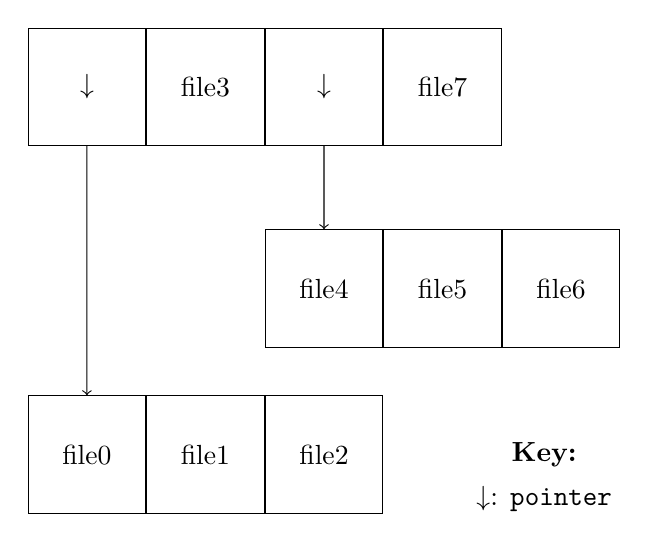
\begin{tikzpicture}[scale=1, square/.style={regular polygon,regular polygon sides=4, minimum width=6em} , x=1cm, y=1cm]
				\node [square,draw] (ptr0) {$\downarrow$};
				\node [square,draw, right=0cm of ptr0] (file3) {file3};
				\node [square,draw, right=0cm of file3] (ptr1) {$\downarrow$};
				\node [square,draw, right=0cm of ptr1] (file7) {file7};
				
				\node [square,draw, below=9em of ptr0] (file0) {file0};
				\node [square,draw, right=0cm of file0] (file1) {file1};
				\node [square,draw, right=0cm of file1 ] (file2) {file2};
				\path [->] (ptr0) edge (file0);
				
				\node [square,draw, below=3em of ptr1] (file4) {file4};
				\node [square,draw, right=0cm of file4] (file5) {file5};
				\node [square,draw, right=0cm of file5] (file6) {file6};
				\path [->] (ptr1) edge (file4);
				
				% Key
				\node [square,right=0cm of file2] (space) {};
				\node [right=0cm of space] (key) {\textbf{Key:}};
				\node [below=0cm of key] (key1) {$\downarrow$: \texttt{pointer}};
			\end{tikzpicture}
		}
	}
	\caption{Example of tree structure for referenced files within a directory\label{fig:b-tree}.}
\end{figure}
% !TeX root = ntfs.tex
\section{Recovery}
\label{sec:Recovery}
After being able to store and organize files it would at first glance seem like the file system is finished, but it is actually quite the opposite: there is a lot more than storing files to a file-system. For example in the event of a crash or power loss the file-system should  try to recover from this crash without losing data or worse completely corrupting the volume or its data. In the following section we will look at how NTFS tries to achieve this crash-protection.

\subsection{Atomic Transactions}
% TODO: Intro sentence
Before analyzing how we can log data to use it for recovery, we will look at how NTFS divides up operations that are to be logged. 
The aforementioned data is broken down into so called \textit{atomic transactions}. In order to understand what atomic transactions are it is easiest to look at the two words separately.\\
A \textit{transaction} is a collection of individual disk and file system operations. An example of an operation could be changing the file name in the MFT entry of the file, whereas the transaction containing this operation would probably also need to update the file-index which points to the file in a directory.\\
Another important concept of  transaction is that a transaction is either complete or incomplete. If it is completed it is said to be \textit{committed}.\\ This leads to the concept of committed projections of a set of transactions: A committed projection of these transaction is the result of the application of only the transactions that have successfully completed (and are henceforth committed). Git is again a good analogy here, as the current \texttt{HEAD}-revision is the committed projection of all changes so far in the repository. NTFS makes sure  that only the committed projections are stored. To accomplish this NTFS caches the changes within a transaction on disk and on completion flushes them to their respective locations.\\
The \textit{atomicity} means that no two different transactions executed at any given time rely on each other. Meaning that each transaction is to be only depended on already committed transactions.


\subsection{Journaling}
In order to be able to recover any data when a crash happens we need to know what the file system was doing when the crash happened. To accomplish this the \textit{Log File Service (LFS)} keeps a \textit{journal} of all transactions occurring. The journal itself is a file (so stored in the MFT) and is usually a less than ten megabytes in size. In order to not fill up the journal file and not be able to log any further transactions, the file is written circularly, which means that once the end of the file is reached, the LFS will continue to write to the journal starting again at the beginning of the file. This means that as soon as this condition sets in, old log records will be overwritten \cite{RUSSINOVICH_ET_AL:2012:WI}, except for if the transactions to be overwritten are not yet committed. In this case NTFS will wait until they are, before executing new transactions\cite{active:NTJ}\\.
In this journal NTFS will record all transactions and especially whether they are committed or not. The transactions recorded undo and redo information for the individual operations within the given transactions.
\subsection{Recovery Process}
After discussing how atomic transactions are recorded, we will now analyze how NTFS uses them to ensure the integrity of the file system in case of a crash. Due to the circular writing and the saving of the current position to write to the journal can be read linearly and due to the atomicity of the transactions, they can be dealt with in the order that they were added.
\paragraph{Analyze:}
Once the system is starting again after a crash, the LFS will seek out all the transactions that were active or incomplete at the time of the crash. These transactions might be breaking the invariant of the file system, that specifies that only completed transactions should be stored.
\paragraph{Redo:}
In the redo-phase, NTFS will make sure all committed transactions are flushed.
As NTFS only wants to keep the committed projections of all transactions, it will not always immediately write to the actual target, but rather keep a on-medium cache of the these changes. They are flushed after committing. In case of a crash these caches might not yet have been flushed to their proper locations, even if transactions are commited, as the crash might have happened between the commit and flush. Hence the LFS will redo these operations and flush them to their appropriate location. 
\paragraph{Undo}
In the undo-phase NTFS will make sure all non-committed transactions are reverted.
After the redo is complete, the LFS will undo all uncommitted transaction, with the idea being that the invariant of only keeping the committed projections must be upheld. For this NTFS will undo all operations in the non-committed transactions. Due to the atomicity of transactions this will work without any conflicts.
\subsection{Redundancy Journal and MFT}
In order to ensure that the two studied vital components of NTFS the journal and the MFT survive crashes, NTFS has built-in redundancies. NTFS for one keeps two copies of the MFT and references them in the boot sector such that if one fails the other one can still be used and a new copy can be built. This is a vital measure that is being taken  as without the MFT the file system is unusable and hence all data on it is corrupt. As of such keeping a copy for redundancy prevents corruption through bad disk sector and through write failures. The journal employs a similar system, only  that there are not two copies of the journal, but rather two pointers to the journal. Using the two pointers it can be ensured that the journal is found again\cite{RUSSINOVICH_ET_AL:2012:WI}. As a missing journal does not mean immediate corruption this seems like a good tradeoff between additional storage requirement and redundancy.
With current disk capacities being as large as they, the choice to only keep to pointers, instead of actually storing two copies, seems questionable. The additional storage requirement for another journal is nearly negligible, but the additional fault tolerance could potentially save the file-system, in case one of the copies is corrupt.
% !TeX root = ntfs.tex
\section{Conclusion}
Modern operating systems need to be able to cope with the ever growing need of storing data. With the \textit{New Technology File  System} Windows can address this problem, by providing a dynamic, scalable and crash-tolerant system for storing and organizing data.
In order to address data on the volume, sectors are grouped into \textit{clusters}, which can then be uniquely referenced. The \textit{Master File Table} stores data and metadata on files, such as the filename, size, and the actual data or references to it. The MFT is organized into a tree structure to represent the file structures a user would employ. In order to be resilient against crashes, NTFS records groups of operations (\textit{transactions}) in a \textit{journal} and will analyze, undo and redo faulty transactions, such that consistency is ensured, as an otherwise corrupt file-system would likely cause data loss to the user.

\bibliographystyle{abbrv}
\bibliography{ntfs}
%\footnotesize
\end{document}
